\section{Entrada y salida}

Un módulo de E/S no es únicamente un conector mecánico quie permite encufar el dispositivo al bus del sistema; sino que además está dotado de cierta <<inteligencia>>, que contiene la lógica necesaria para permitir la comunicación entre el periférico y el bus.

Las razones por las que los periféricos no se conectan directamente al bus del sistema son:

\begin{itemize}
  \item Hay una plia variadadd e periféricos con formas de funcionamiento direferentes. Podría ser imposible incorporar la lógica necesaria dentro del procesador para controlar tal diversidad de dispositivos.
  \item Generalmente, la velocidad de transferencia de datos de los periféricos es mucho menor que la de la memoria o el procesador.
  \item Por otro lado, la velocidad de transferencia de algunos periféricos es mayor que la de la memoria o el procesador.
  \item Los periféricos suelen utilizar datos con formatos y tamaños de palabra diferentes de los del computador a los que se conectan.
\end{itemize}

En consecuencia, se necesita un módulo de E/S. Este módulo tiene dos funciones principales:

\begin{itemize}
  \item Realizar la interfaz entre el procesador y la memoria y los periféricos.
  \item Realizar la interfaz entre uno o más dispositivos periféricos.
\end{itemize}

\subsection{Dispositivos externos}

Un dispositivo externo se conecta al computador mediante un enlace a un módulo de E/S. El enlace se utiliza para intercambiar señales de control, estado, y datos entre el módulo de E/S y el dispositivo externo. Los dispositivos externos pueden ser:

\begin{itemize}
  \item \textbf{E/S básicos}: monitor, mouse, teclado, etc.
  \item \textbf{E/S de almacenamiento}: discos duros, CD-ROM, etc.
  \item \textbf{Impresión}: impresoras, escáneres, etc.
  \item \textbf{Comunicaciones}: módems, acceso/interfaz de red, etc.
  \item \textbf{Multimedia}: microfónos, altavoces, etc.
  \item \textbf{Automatización y control}: sensores, alarmas, etc.
\end{itemize}

\begin{figure}[H]
  \centering
  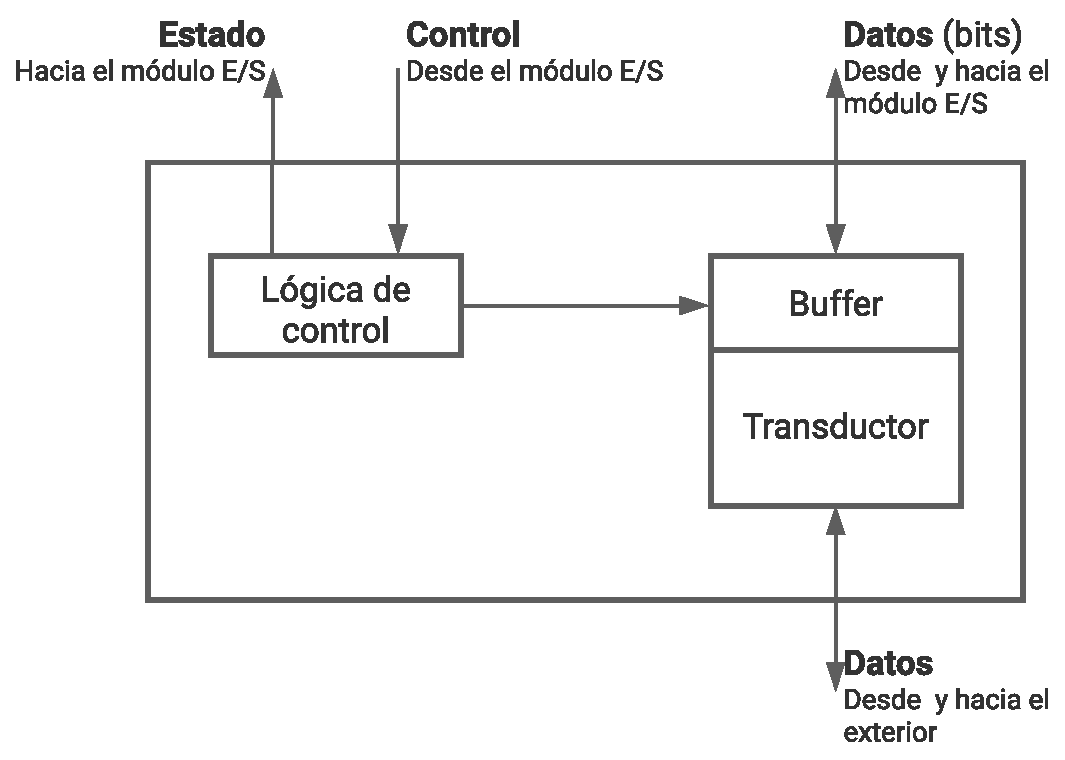
\includegraphics[width=0.6\textwidth]{Dispositivo-externo-tipo}
  \caption{Dispositivo externo}\label{fig:Dispositivo-externo-tipo}
\end{figure}

La forma de un dispositivo externo se indica en la Figura~\ref{fig:Dispositivo-externo-tipo}. La conexión con el módulo de E/S se realiza a través de señales de control, estado y datos. 

La \textit{lógica de control} asociada al dispositivo controla su operación en respuesta a las indicaciones del módulo de E/S. El \textit{transductor} convierte las señales eléctricas asociadas al dato a otra forma de energía en el caso de una salida y viceversa en el caso de unta entrada. Existe un buffer asociado al transductor para almacenar temporalmente el dato que se esta transfiriendo ente el módulo de E/S y el exterior.

\subsection{Funciones de un módulo de E/S}

Las principales funciones y requisitos de un módulo de E/S se esncuentran dentro de las siguientes categorías:

\begin{itemize}
  \item \textbf{Control y temporización}: coordina el tráfico entre los recursos internos y los dispositivos externos.
  \item \textbf{Comunicación con el procesador}: implica la decodificación de órdenes, el intercambio de datos, información del Estado y el reconocimiento de direcciones.
  \item \textbf{Comunicación con los dispositivos}: esta comunicación implica intercambiar órdenas, información del estado y datos.
  \item \textbf{Almacenamiento temporal de datos}: los datos que se transfieren entre el módulo de E/S y los dispositivos externos se almacenan temporalmente en un buffer.
  \item \textbf{Detección de errores}: detecta los errores e informa al procesador.
\end{itemize}

La complejidad de los módulos de E/S y el número de dispositivos externos que controlan varían considerablemente. 

El funcionamiento de un módulo de E/S permite que el procesador vea a una amplia gama de dispositivos de forma simplificada. El módulo debe ovultar los detalles de temporización, formatos y electromecanica de los dispositivos externos para que el procesador pueda funcionar únicamente en términos de órdenes de lectura y escritura.

Un módulo de E/S que se encarga de la mayoría de los detalles del procesamiento, presentando al procersador una interfaz de alto nivel, se denomina \textit{canal de E/S} o \textit{procesador de E/S}. Un módulo que sea bastante simple qy requiera control detallado normalmente se denomina \textit{controlador de E/S}.

\begin{figure}[h]
  \centering
  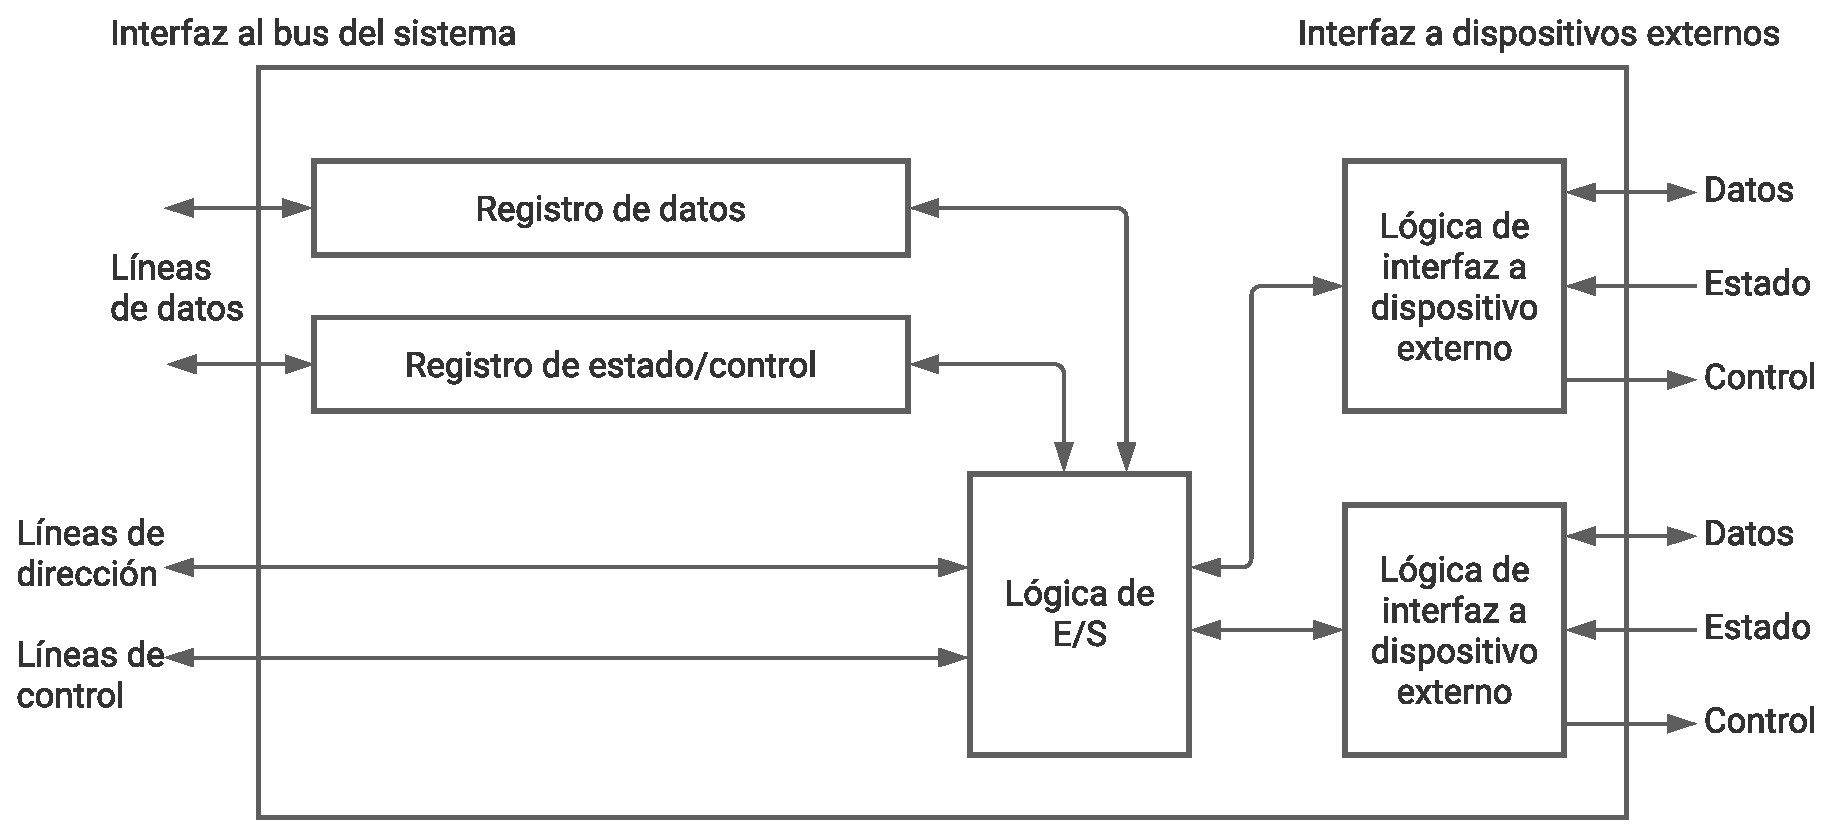
\includegraphics[width=0.6\textwidth]{Modulo-IO}
  \caption{Estructura de un módulo de E/S}\label{fig:Estructura-modulo-E/S}
\end{figure}